\documentclass[9pt,a4paper,twocolumn,twoside]{tau-class/tau}
\usepackage[ngerman]{babel}

% Titel & Metadaten
\journalname{Handout}
	\title{Space Radiation Effects in Electronics}

\author[a,1]{Florian Marius Adamczyk}
\affil[a]{Justus-Liebig-Universität Gießen}
\professor{Modul Wissenschaftliches Präsentieren}

% Footer-Informationen
\institution{JLU Gießen}
\footinfo{Weltraumstrahlungseffekte in der Elektronik}
	\theday{\today}
\leadauthor{Adamczyk}
\course{Wissenschaftliches Präsentieren}
% Bibliographie
\usepackage{csquotes}
\addbibresource{references.bib}

% Grafiken
\usepackage{graphicx}
\graphicspath{{Images/}}

\begin{abstract}
Dieses Handout fasst die wichtigsten Inhalte der Präsentation \enquote{Space Radiation Effects in Electronics} zusammen. Im Fokus stehen die Grundlagen kumulativer Strahlungsschäden (TID), die Strahlungsumgebung im Orbit, der physikalische Mechanismus im MOS-Bauelement, funktionale Konsequenzen in Schaltungen sowie Test- und Qualifikationsverfahren (RHA).
\end{abstract}

\keywords{Total Ionizing Dose, MOS, Raumfahrt, RHA, TID-Tests}

\begin{document}

\maketitle
	\thispagestyle{firststyle}
	\tauabstract

\section{Einordnung der Strahlungseffekte}
	\taustart{S}trahlungseffekte in Elektronik lassen sich grob in zwei Klassen einteilen: (i) kumulative Effekte wie \textbf{Total Ionizing Dose (TID)} und \textbf{Displacement Damage (DDD)}, die dosisabhängig und langsam wirken; und (ii) \textbf{Single Event Effects (SEE)} wie SEU/SEL/SEB/SEGR, die durch Einzelereignisse verursacht werden und spontan auftreten. TID steht im Zentrum dieses Handouts, da sie nahezu alle Technologien betrifft und langfristig zu Parameterverschiebungen und Degradation führt.

\section{Strahlungsumgebung}
\subsection{Quellen im Weltraum}
Relevante Quellen sind die \textbf{Sonne} (solare Protonenereignisse), die \textbf{Van-Allen-Gürtel} (gefangene Protonen und Elektronen) sowie \textbf{GCR} (galaktische kosmische Strahlung). Für TID tragen vor allem \textbf{Elektronen und Protonen} bei; Photonen und sekundäre Elektronen ergänzen den Beitrag \parencite{esa_radiation_rangers_2024}.

\begin{figure}[h]
  \centering
  \includegraphics[width=0.7\columnwidth]{image-4_upscayl_2x_digital-art-4x.png}
  \caption{Illustration kosmischer Strahlungsquellen \parencite{esa_radiation_rangers_2024}.}
\end{figure}

\subsection{Südatlantische Anomalie (SAA)}
Die SAA ist ein Gebiet mit lokal geschwächtem Erdmagnetfeld, in dem erhöhte Flüsse von MeV-Protonen und -Elektronen auftreten. Satelliten in LEO durchqueren die Region regelmäßig; die \textbf{Dosis akkumuliert} über die Missionsdauer und kann je nach Orbit und Abschirmung \textbf{zweistellige krad(Si)} erreichen \parencite{esa_saa_2025}.

\begin{figure}[h]
  \centering
  \includegraphics[width=0.95\columnwidth]{South_Atlantic_Anomaly_2025_compared_to_2014.jpg}
  \caption{Südatlantische Anomalie \parencite{esa_saa_2025}.}
\end{figure}

\section{TID-Mechanismus im MOS}
\subsection{Ionisation im Oxid}
Ionisierende Strahlung erzeugt \textbf{Elektron-Loch-Paare} im SiO$_2$-Gateoxid. Aufgrund der \textbf{geringen Lochmobilität} werden Löcher in \textbf{Defektstellen (Traps)} eingefangen (z.B. Oxygen Vacancies, E'-Center), während Elektronen schnell entweichen. Es entsteht eine \textbf{persistente positive Raumladung} im Oxid \parencite{Sanchez_Esqueda_2015_compact_modeling_TID}.

\begin{figure}[h]
  \centering
  \includegraphics[width=0.95\columnwidth]{transistor_h-e_upscayl_4x_digital-art-4x.png}
  \caption{Schema: Erzeugung und Trapping von Ladungsträgern im Gateoxid \parencite{Sanchez_Esqueda_2015_compact_modeling_TID}.}
\end{figure}

\subsection{Auswirkungen auf Transistor}
Die Oxidladung verschiebt die \textbf{Schwellenspannung} ($V_{th}$): bei NMOS sinkt $V_{th}$, der Kanal leitet früher; Leckströme steigen, der Subthreshold-Bereich wird flacher. Bei PMOS sind die Vorzeichen oft umgekehrt \parencite{7776909}.

\begin{figure}[h]
  \centering
  \includegraphics[width=0.95\columnwidth]{EffectsOnTransistor_upscayl_5x_digital-art-4x.png}
  \caption{Auswirkungen auf I--V-Kennlinien und Parameter \parencite{7776909}.}
\end{figure}

\section{Funktionale Konsequenzen}
Auf Schaltungsebene führt TID zu \textbf{Timing-Änderungen} und langsameren Schaltzeiten, zu \textbf{erhöhten Ruheströmen} und \textbf{Mismatch} in Analogschaltungen (Offsets, Verstärkungsänderungen). Langfristig \textbf{driften Bauteile aus der Spezifikation} und können ausfallen. In digitalen Schaltungen verschieben sich Logikpegel und \textbf{Noise-Margen} werden schlechter.

\section{Tests und Qualifikation (RHA)}
\subsection{Ziele der RHA}
Für Raumfahrt-Elektronik muss nachgewiesen werden, dass Bauteile unter der \textbf{Missionsdosis} funktionsfähig bleiben. Zielgrößen sind u.a. $\Delta V_{th}$, Leckströme und Funktionsgrenzen (Logikpegel, analoge Spezifikationen) \parencite{calebnstxl_2022_strengthening_reliability}.

\subsection{TID-Testquellen und Randbedingungen}
Typische Quellen sind \textbf{Co-60-Gammastrahler} (1{,}17/1{,}33 MeV) und \textbf{Elektronen} ($E\geq$ 1 MeV). Gründe: hohe \textbf{Penetration} und \textbf{homogene Dosis} bei geringer DDD-Komponente. Nach Normen (z.B. ESCC 22900) werden geeignete \textbf{Dosisraten} gewählt und \textbf{Charged-Particle Equilibrium} sichergestellt; Low-Energy-Anteile werden durch \textbf{Pb/Al-Abschirmung} reduziert.

\section{Kernaussagen}
\begin{itemize}
  \item \textbf{TID} ist ein kumulativer Ionisationsschaden in \textbf{Oxiden/Grenzflächen}.
  \item Hauptmechanismus: \textbf{Oxid-trapped charge} $\Rightarrow \Delta V_{th}$, Mobility-Degradation, Leckstrom $\uparrow$.
  \item Bauteile \textbf{driften aus Spezifikation} bis zum Funktionsverlust.
  \item \textbf{RHA/TID-Tests} sind unverzichtbar für Weltraummissionen.
\end{itemize}

\section{Telstar 1: Aufstieg und abruptes Ende}
Der Kommunikationssatellit \textbf{Telstar 1} startete am 10. Juli 1962 und ermöglichte die ersten transatlantischen Live--Fernsehübertragungen. Kurz darauf traten jedoch Anomalien auf: Befehle wurden sporadisch ignoriert, bis der Satellit am 21. Februar 1963 endgültig ausfiel. Als wesentlicher Beitrag zur Degradation gilt die \textbf{kumulative Ionisationsdosis (TID)}, die durch die am Vortag des Starts durchgeführte Hochatmosphärenkernexplosion \textbf{Starfish~Prime} stark erhöht wurde \parencite{bbc_2024_first_live_telstar,atomicarchive_fishbowl_1962}.

\begin{figure}[H]
  \centering
  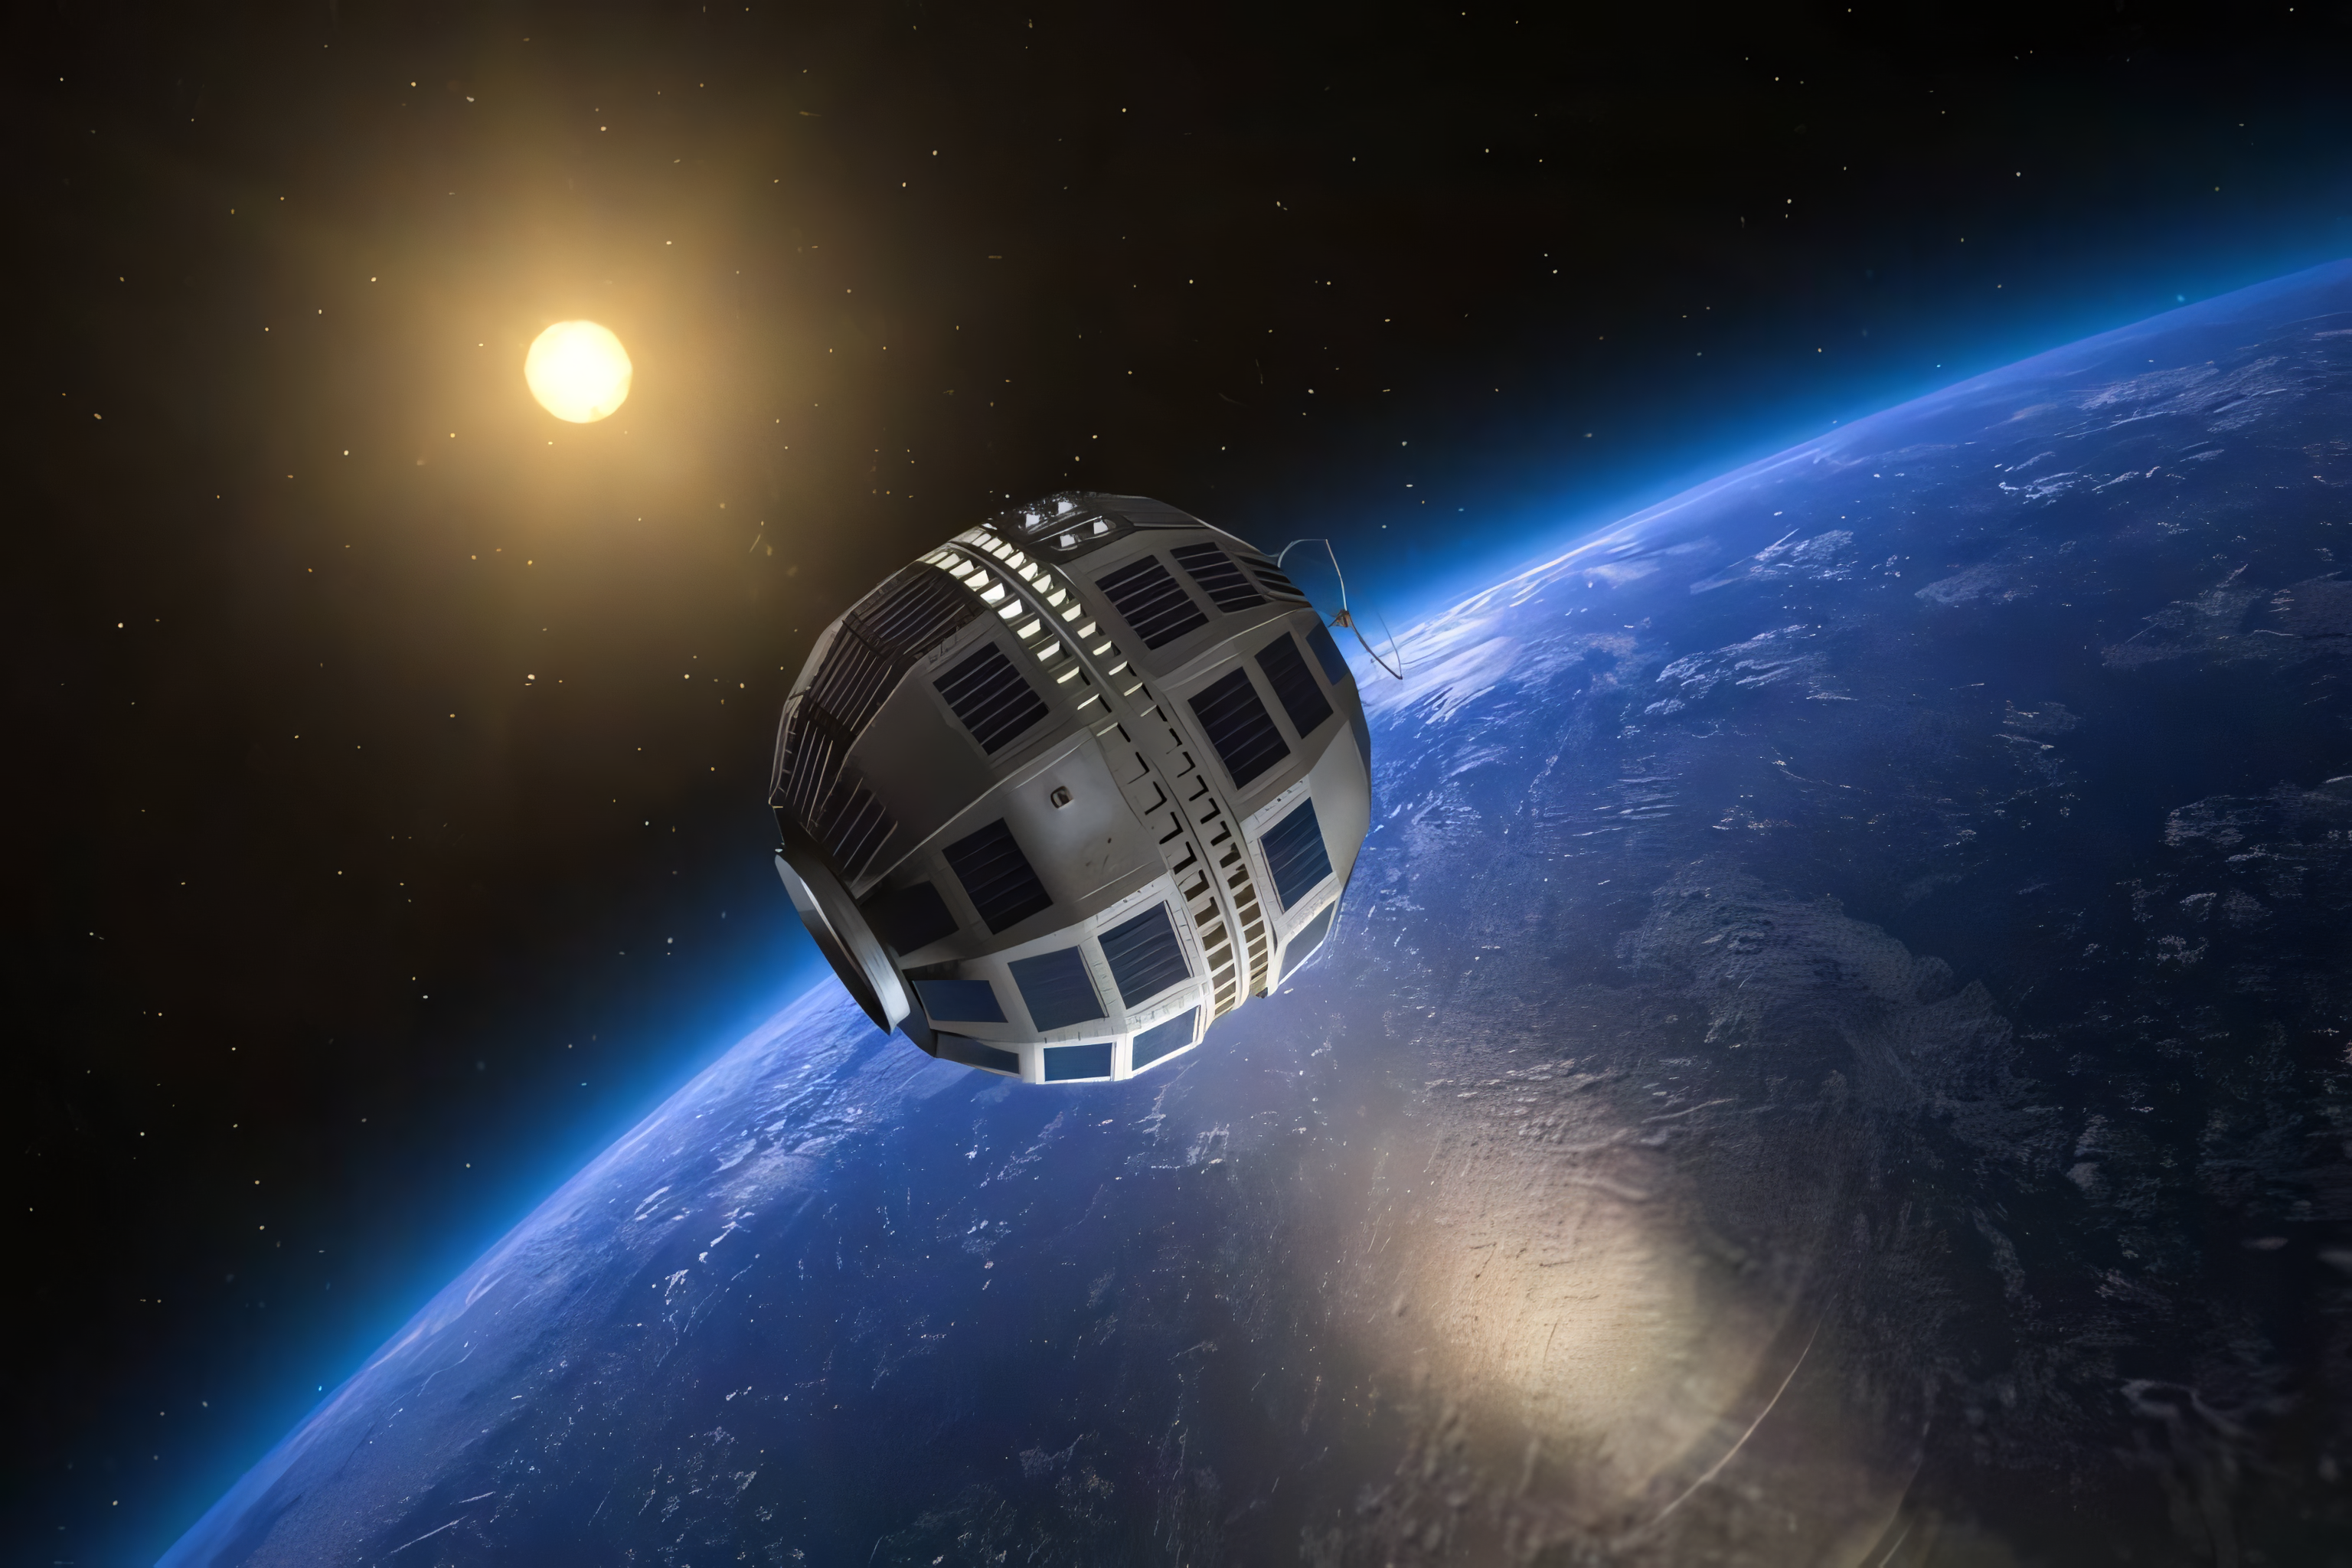
\includegraphics[width=0.95\columnwidth]{Telstar1_upscayl_4x_ultramix-balanced-4x.png}
  \caption{Telstar 1 -- Symbol der ersten transatlantischen TV--Live--Übertragung \parencite{adobe_174965630_2025,bbc_2024_first_live_telstar}.}
\end{figure}

\begin{figure}[H]
  \centering
  \includegraphics[width=0.6\columnwidth]{Fishbowl-Starfish-Prime-5.jpg}
  \caption{Starfish Prime (1962): Hochatmosphärischer Nukleartest und verstärkte Strahlungsgürtel \parencite{atomicarchive_fishbowl_1962}.}
\end{figure}

% \section{Abbildungen}
% Die in der Präsentation gezeigten Illustrationen und Fotos stammen aus den genannten Quellen, u.a. \parencite{esa_radiation_rangers_2024,esa_saa_2025,7776909,Sanchez_Esqueda_2015_compact_modeling_TID,calebnstxl_2022_strengthening_reliability}. Zusätzliche Einleitungsbilder: \parencite{10843774,delta_rocket_telstar1_46898,adobe_174965630_2025,atomicarchive_fishbowl_1962}.

%----------------------------------------------------------
\printbibliography
%----------------------------------------------------------

\end{document}